\documentclass[a4paper,12pt,abstracton]{scrartcl}
\usepackage[utf8]{inputenc}
\usepackage{float}
\usepackage{amsmath}
\usepackage{amssymb}
\usepackage{pifont}% http://ctan.org/pkg/pifont
\usepackage[font=small,labelfont=bf]{caption}
\usepackage{graphicx}
%\usepackage{dirtytalk}
\usepackage{multicol}
\usepackage{booktabs}
\usepackage{colortbl}
\usepackage{appendix}
\usepackage{nomencl}
\usepackage{lmodern}
\usepackage[nottoc]{tocbibind}
\usepackage{xcolor}
%\graphicspath{images/}
\usepackage[margin = 3cm]{geometry}
\usepackage{ragged2e} % good alignment
\usepackage{hyperref}
\usepackage{siunitx} % Provides the \SI{}{} and \si{} command for typesetting SI units
\hypersetup{colorlinks=true,
    linkcolor=blue,
    filecolor=magenta,      
    urlcolor=cyan, 
    citecolor=gray}

%\DeclareGraphicsExtensions{.png,.pdf} % low-res (work in progress)
%\DeclareGraphicsExtensions{.pdf,.png}  % high-res (final draft)
%\setlength\parindent{0pt} % Removes all indentation from paragraphs
%\bibliographystyle{unstr}
\setlength\parindent{0pt}
\setlength{\parskip}{0.3em}
\newcommand{\xmark}{\ding{55}}

\renewcommand{\nomname}{List of Symbols}
\renewcommand{\nompreamble}{The following list explains the symbols used within the body of the report.}

\usepackage{etoolbox}
\renewcommand\nomgroup[1]{%
  \item[\bfseries
  \ifstrequal{#1}{E}{Experimental Equipment}{%
  \ifstrequal{#1}{C}{Computational Methods}{%
  \ifstrequal{#1}{T}{Theoretical Concepts}{
  \ifstrequal{#1}{P}{Physical Constants}{}}}}%
]}


\subject{CMP Lab Report} % Matter Physics, Physics, Chemical Physics ?
\title{Zeeman Effect}
\author{Group B9\footnote{Pietro Monticone , Claudio Moroni , Alberto Mosso , Riccardo Valperga.}}

\renewcommand{\listfigurename}{Plots}
\renewcommand{\listtablename}{Tables}
\renewcommand{\nomname}{Nomenclature}


\begin{document}
\maketitle
\makenomenclature
\newpage
\section{Magnetic Field Uniformity check}
As stated in the introduction, one has to check quantitatively whether the magnetic field between the expansion is uniform, in order to associate to it a proper uncertainty. We took 5 measures of $B$ between the expansions along a horizontal diameter and 5 along a vertical one.\newline
The horizontal data collected are:
\begin{table}[H]
\centering
\caption{}
\label{disX}
\resizebox{10cm}{!}{
\begin{tabular}{ccc}
\toprule
$I\;[A]$ & $x$ [mm] & $B\;[T]$       \\
\midrule
\rowcolor{gray!6}  4.20 $\pm$ 0.02 & -10.23 $\pm$ 0.05 & 0.248 $\pm$ 0.001 \\
 & -7.10 $\pm$ 0.05 & 0.278 $\pm$ 0.001 \\
\rowcolor{gray!6}   & -4.15 $\pm$ 0.05 & 0.285 $\pm$ 0.001 \\
 & 0.00 $\pm$ 0.05 & 0.285 $\pm$ 0.001 \\
\rowcolor{gray!6}   & 4.15 $\pm$ 0.05 & 0.285 $\pm$ 0.001 \\
 & 7.10 $\pm$ 0.05 & 0.278 $\pm$ 0.001 \\
\rowcolor{gray!6}   & 10.23 $\pm$ 0.05 & 0.247 $\pm$ 0.001 \\
\bottomrule
\end{tabular}}
\end{table}

\begin{figure}[H]
\begin{center}
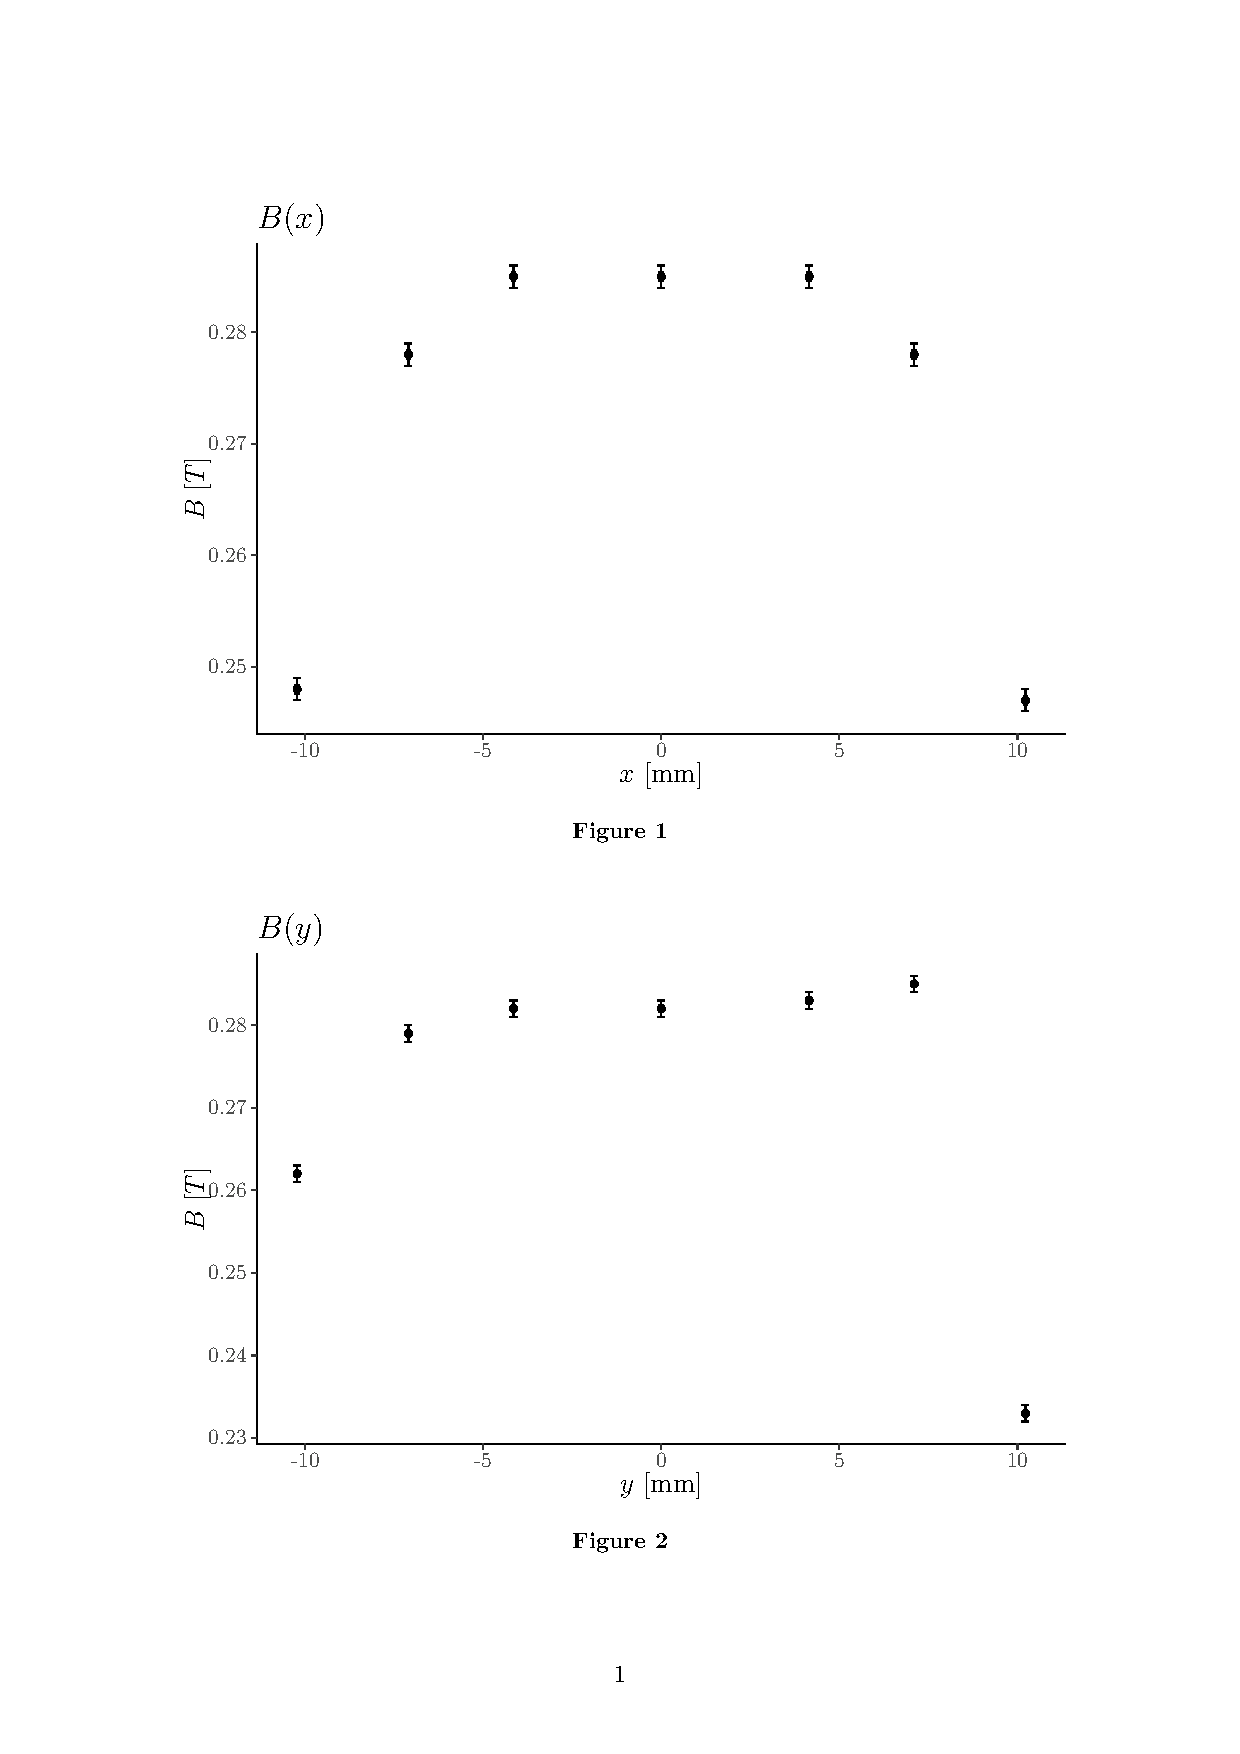
\includegraphics[trim=3cm 15cm 3cm 3cm, clip,height=9cm,keepaspectratio]{MagneticDishomogeneity.pdf}
\end{center}
\end{figure}

Because the spectroscopic lamp was taller than larger, only the first four measures around the central position have been taken into account to evaluate the horizontal uncertainty. This has been calculated as the maximum half-dispersion.$$MHD_{hor}=0.007 \; T$$
The vertical uncertainty has been computed as the maximum half-dispersion again, but this time we considered all measurements:
\begin{table}[H]
\centering
\caption{}
\label{disY}
\resizebox{10cm}{!}{
\begin{tabular}{ccc}
\toprule
$I\;[A]$ & $y$ [mm] & $B\;[T]$       \\
\midrule
\rowcolor{gray!6}  4.13 $\pm$ 0.02 & -10.23 $\pm$ 0.05 & 0.262 $\pm$ 0.001\\
 & -7.10 $\pm$ 0.05  & 0.279 $\pm$ 0.001\\
\rowcolor{gray!6}   & -4.15 $\pm$ 0.05 & 0.282 $\pm$ 0.001\\
 & 0.00 $\pm$ 0.05 & 0.282 $\pm$ 0.001\\
\rowcolor{gray!6}   & 4.15 $\pm$ 0.05 & 0.283 $\pm$ 0.001\\
 & 7.10 $\pm$ 0.05 & 0.285 $\pm$ 0.001\\
\rowcolor{gray!6}   & 10.23 $\pm$ 0.05 & 0.233 $\pm$ 0.001\\
\bottomrule
\end{tabular}}
\end{table}

\begin{figure}[H]
\begin{center}
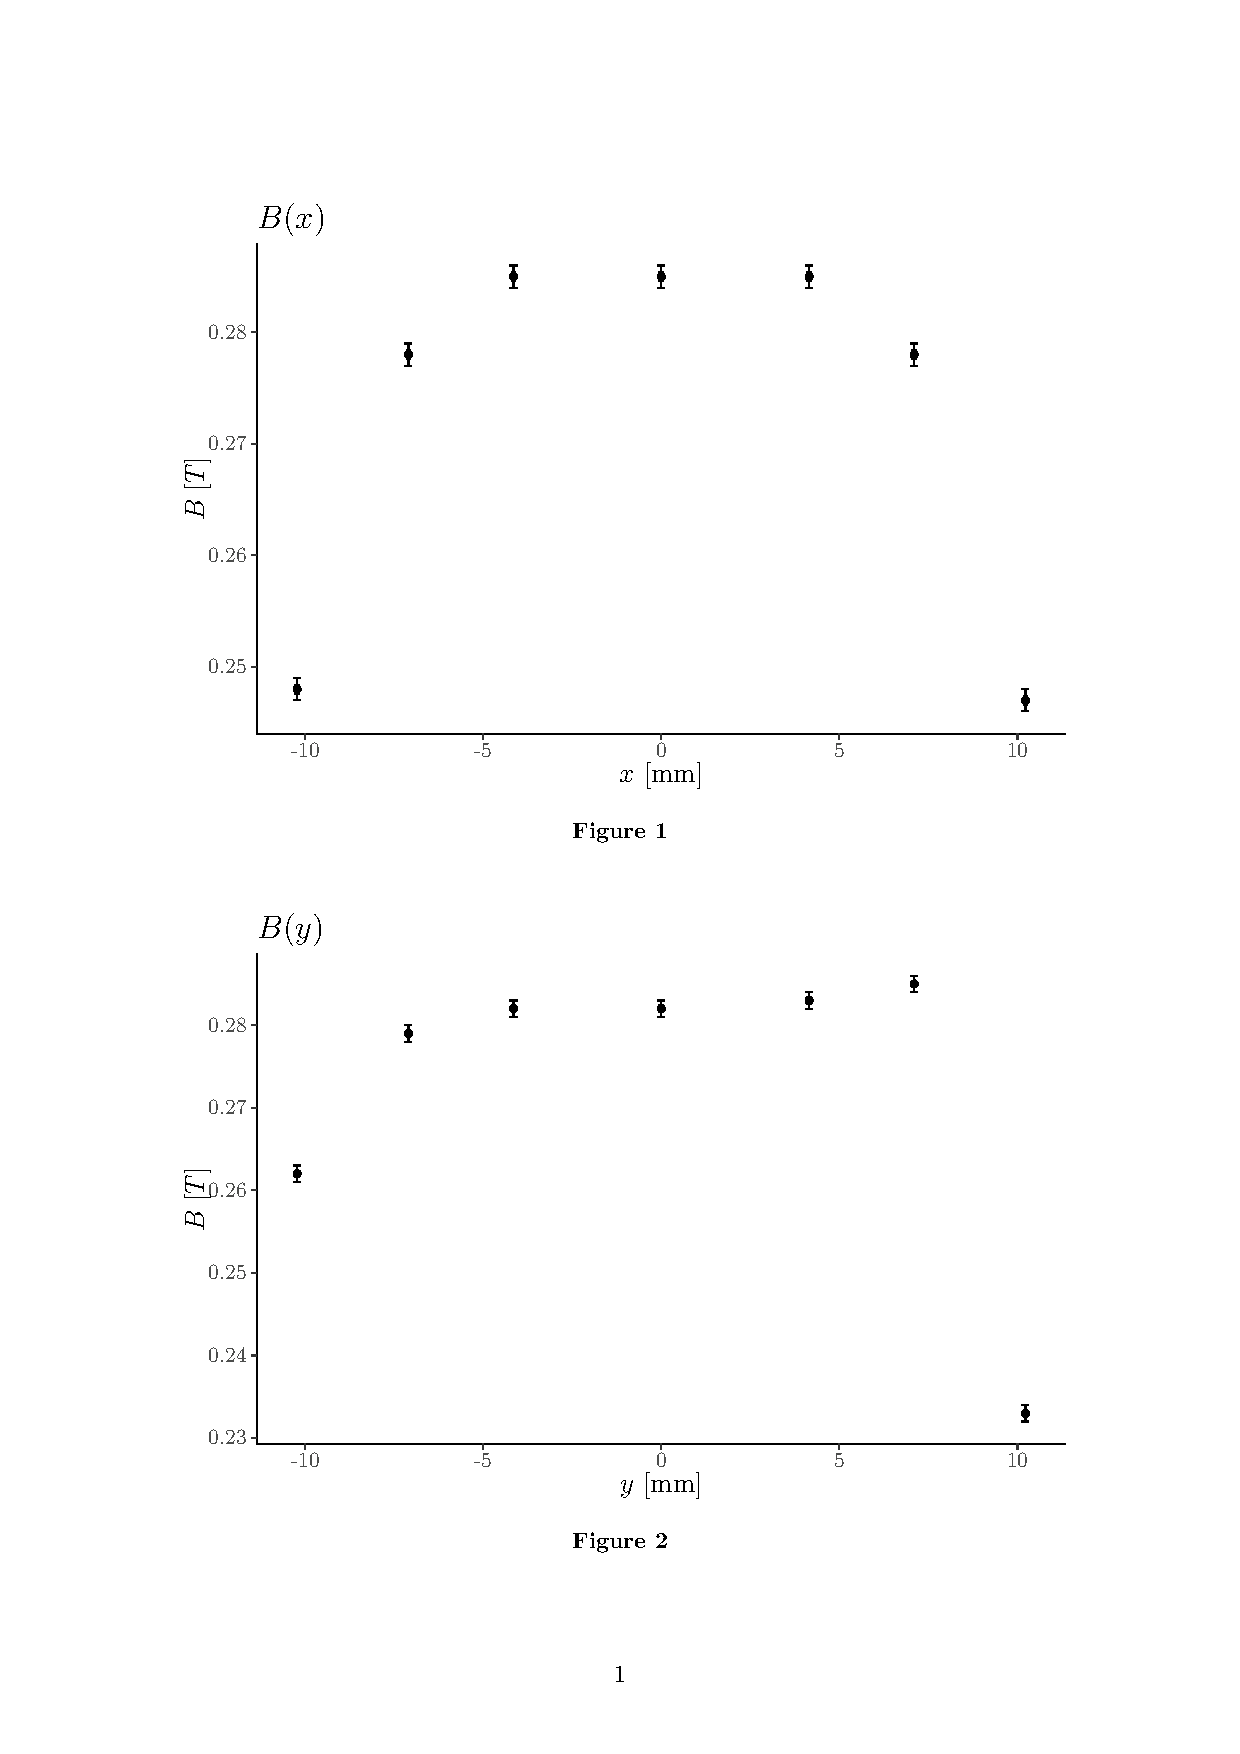
\includegraphics[trim=3cm 4cm 3cm 15cm, clip,height=9cm,keepaspectratio]{MagneticDishomogeneity.pdf}
\end{center}
\end{figure}
$$MHD_{ver}=0.052 \; T$$
An average of the two half-dispersion has been made, and the relative error (with respect to the maximum measurement 0.285 T) computed:

\begin{table}[H]
\centering
\caption{}
\label{disY}
\resizebox{10cm}{!}{
\begin{tabular}{cccc}
\toprule
$MHD_{hor}$ & $MHD_{ver}$ & $average$ & $Relative \; Error$       \\
\midrule
\rowcolor{gray!6} 0.007 T & 0.052 T & 0.0295 T & 0.1035087719\\
\bottomrule
\end{tabular}}
\end{table}

In the following sections, we will use the product between the relative error and the measured value of B as the error to be associated to the magnetic field, unless the propagation using the calibration curve yields a larger value. 

\end{document}
